\let\negmedspace\undefined
\let\negthickspace\undefined
\documentclass[a4,12pt,onecolumn]{IEEEtran}
\usepackage{amsmath,amssymb,amsfonts,amsthm}
\usepackage{algorithmic}
\usepackage{graphicx}
\usepackage{textcomp}
\usepackage{xcolor}
\usepackage{txfonts}
\usepackage{listings}
\usepackage{enumitem}
\usepackage{mathtools}
\usepackage{gensymb}
\usepackage[breaklinks=true]{hyperref}
\usepackage{tkz-euclide}
\usepackage{listings}
\usepackage{circuitikz}
\usepackage{gvv}
\begin{document}
\title{
\Huge\textbf{ GATE 2023 Assignment}\\
\Huge\textbf{EE1205} Signals and Systems\\
}
\large\author{Kurre Vinay\\EE23BTECH11036}
\maketitle
\textbf{Question(IN 46):}
In the circuit shown ,$\omega=100\pi\text{rads/s}$, R1=R2=$2.2\Omega$ and L=$7\text{mH}$. the capacitance $\text{C}$ for which $Y_{in}$ is purely real is  $\text{mF}$ \\
	\vspace{0.3cm}
	\begin{center}
	\begin{circuitikz} \centering \draw 
		(0,4) to[sinusoidal voltage source, l=$V_{0}$cos($\omega$t)] (0,0)
		(0,4) to[short] (4,4)
		(4,4) to[resistor, l=$R_1$ ] (4,2)
		(4,2) to[inductor, l= $\text{L} $] (4,0) to[short ] (0,0)
		(8,4)  to[short] (4,4)
		(8,4) to[resistor, l= $R_2$] (8,2) to[capacitor,l=$\text{C}$] (8,0) to (4,0)
		;
	\end{circuitikz}
	\end{center}
\hfill(GATE ST 2023)\\
\solution
\begin{table}[ht!]
 \begin{center}
\begin{tabular}{|c|c|c|}
   \hline
   variable&value&description  \\
   \hline
   $Y_{in}$ & & Admittance of circuit\\
   \hline
   $X_{L}$ & $7s\Omega$ & Inductive reactance \\
   \hline
   $X_{C}$ &$\frac{1}{s\text{C}}\Omega $ & Capacitive reactance \\
   \hline
   $\omega$ &$100\pi$rads/s& Angular frequency\\
   \hline
\end{tabular}
\caption{Table: Input Parameters}
\end{center}
\end{table}
\begin{align}
X_L&=\text{sL}\\
&= 7s\Omega\\
X_C&=\frac{1}{s\text{C}}\Omega\\
Y_{in}&=\frac{1}{2.2+7s} + \frac{1}{2.2+\frac{1}{ \text{sC}}}\\
s&=j\omega \\
\implies  Y_{in}&=\frac{1}{2.2+7j\omega} + \frac{1}{2.2+\frac{1}{j\omega \text{C}}}\\
\implies  Y_{in}&=\frac{1-j}{4.4} + \frac{2.2+\frac{j}{\omega\text{C}}}{(2.2)^2+\brak{\frac{1}{\omega\text{C}}}^2}
\end{align}
According to the question given, $Y_{in}$ is purely real , so imaginary part should be equal to zero\\
\begin{align}
&\implies  \frac{-1}{4.4}+\frac{\frac{1}{\omega\text{C}}}{(2.2)^2+\brak{\frac{1}{\omega\text{C}}}^2} = 0\\
&\implies  \frac{\frac{1}{\omega\text{C}}}{(2.2)^2+\brak{\frac{1}{\omega\text{C}}}^2}=\frac{1}{4.4}\\
&\implies  (2.2)^2-\frac{4.4}{\omega\text{C}}+\brak{\frac{1}{\omega\text{C}}}^2=0\\
&\implies  \brak{2.2-\frac{1}{\omega\text{C}}}^2=0\\
&\implies  \frac{1}{\omega\text{C}}=2.2\\
&\implies  \text{C}=\frac{700}{484}\text{mF}\\
&\implies  \text{C}=1.446281\text{mF}
\end{align}
The capacitance of capacitor $\text{C}$ is 1.45$\text{mF}$
\begin{figure}[ht!]
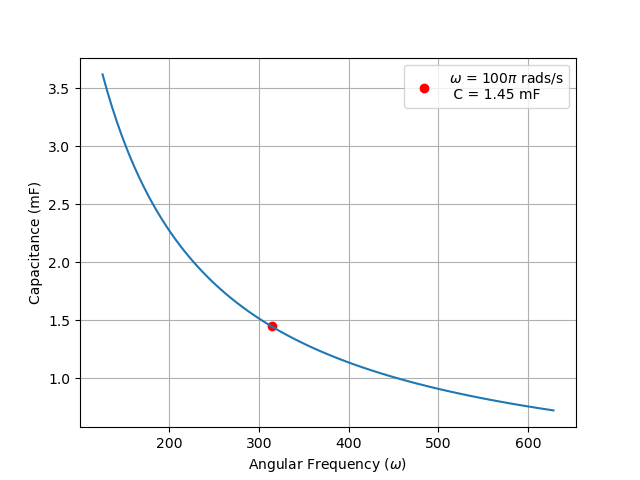
\includegraphics[width=\columnwidth]{fig/fig3.png}
\caption{Graph of Capacitance($\text{mF}$) vs Angular Frequency($\omega$)}
\end{figure}
\end{document}
